%!TEX root = main.tex
\section{Conclusion} % (fold)
\label{sec:conclusion}
This experiment was designed to investigate two phenomena using a Beryllium-Americium source and a pair of nuclear detectors. The first was to make a measurement of the binding energy of the deuteron by observing the $\gamma$-ray emitted when neutrons are captured by protons in the water surrounding a neutron source via the reaction 
\begin{align}
	p + n \rightarrow d + \gamma.
\end{align}
This was found to have a value of 2.2245\,MeV which is very close to the accepted value of $2224.52\pm 0.20$\,keV. The measurement of the deuteron binding energy was very successful, however, the preliminary experiments to investigate the detector itself, to determine its energy resolution and efficiency by looking at samples with known well defined peaks was less successful. 

Problems were encountered when plotting the data that had been acquired suggesting that it was not accurate enough to draw any firm conclusions possibly because of the errors that had been introduced during measurement. There was often a general trend in the data as would be expected, but the points were too scattered to be able to fit the data to the mathematical model. For example, when looking at the efficiency of the sodium iodide detector, the plot in figure~\ref{fig:NaIefficiancy} was measured.
\begin{figure}[ht]
	\centering
	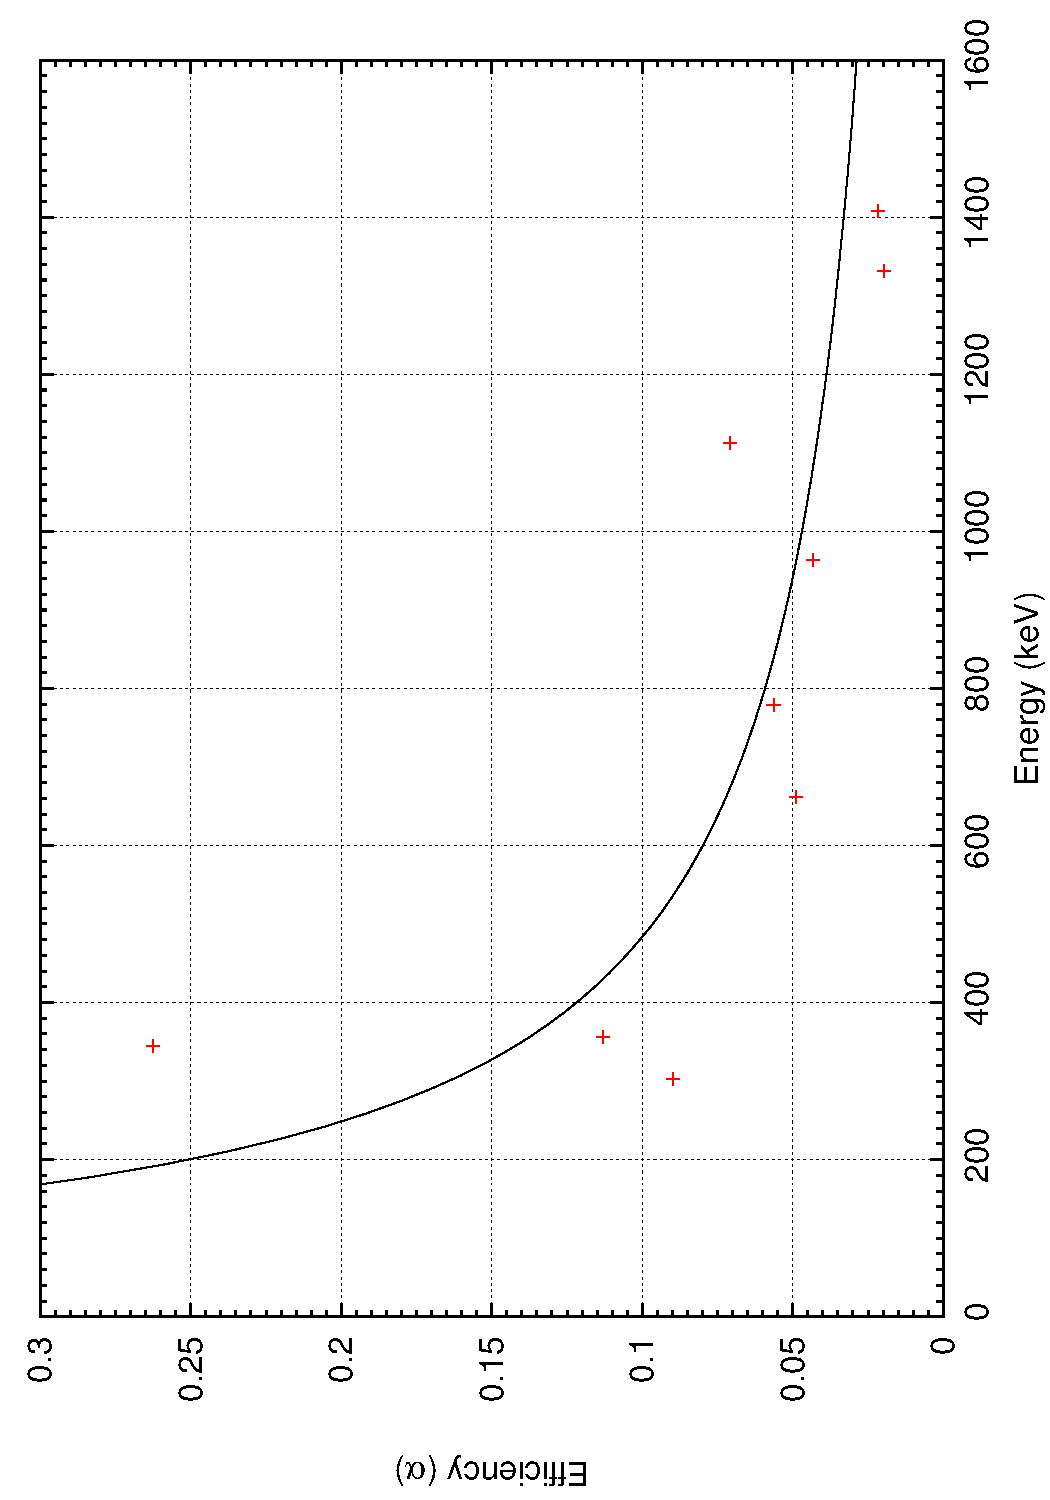
\includegraphics[angle=270,width=0.6\textwidth]{NaIEfficiency.pdf}
	\caption{The sodium iodide detector provides a channel number readout that is directly proportional to the energy of the corresponding reaction event. Thus, using known data points, a relation between channel number and energy can be found.\label{fig:NaIefficiancy}}
\end{figure}
Though this is a poor fit, as the data points are not closely matched to the line, we can confirm that the general trend in the efficiency as the energy increases is correct, as can be seen in the diagram in figure~\ref{fig:efficiencyKrane}\cite{krane}.
\begin{figure}[ht]
	\centering
	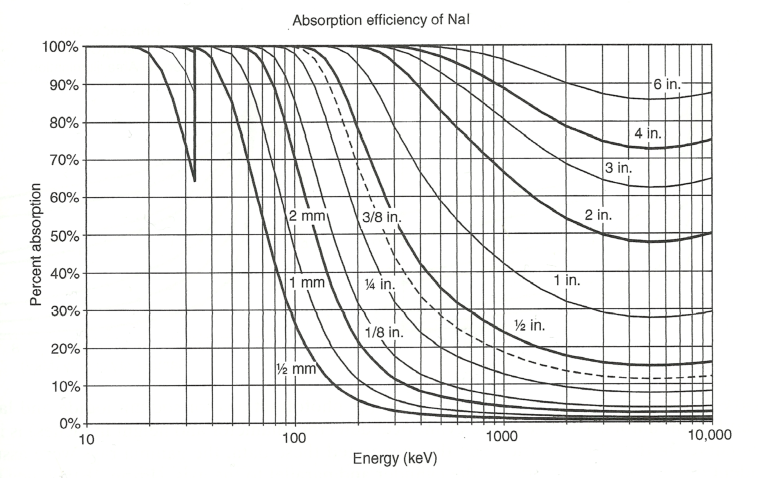
\includegraphics[width=0.7\textwidth]{EfficiencyKrane.pdf}
	\caption{The sodium iodide detector provides a channel number readout that is directly proportional to the energy of the corresponding reaction event. Thus, using known data points, a relation between channel number and energy can be found.\label{fig:efficiencyKrane}}
\end{figure}

The second experiment involved using a boron triflouride detector to measure the moderating effect of water on the neutrons observed from a BeAm source. For this we found that there were several elements of the spectra that were observed that had to be understood in order to measure the moderating effects fully. These included the wall effect and the contribution of the background radiation to the readings made by the proportional counter. 

Once these elements were understood, we were able to take measurements of the neutron flux at increasing radii from the source, moving out through the tank filled with water. We found that the majority of the data followed the expected trend provided by the one-group equation describing the thermalization of neutrons in the water tank.
% section conclusion (end)
